\documentclass[12pt]{article}

% Paquetes necesarios
\usepackage[utf8]{inputenc}
\renewcommand{\rmdefault}{ptm}
\usepackage[T1]{fontenc}
\usepackage[spanish]{babel}
\usepackage{graphicx}
\usepackage{caption}
\usepackage{titling}   % Permite personalizar el título
\usepackage{geometry}  % Controla márgenes
\usepackage{multicol}  % Permite columnas
\usepackage{hyperref}
\usepackage{float}
\usepackage{booktabs}


% Márgenes personalizados
\geometry{margin=2.5cm}


\title{\Huge Informe de Trabajo Final\\Visión por Computadora III - CEIA}
\newcommand{\subtitle}{\Large Traducción de Imágenes a Texto}

\begin{document}


\begin{center}
    {\small \today}  %  fecha actual
\end{center}

% Imagen arriba del título
\begin{figure}[t]
    \centering
    
\includegraphics[width=0.8\textwidth]{../reports/figures/logoFIUBA.pdf}
\end{figure}

% Título y subtítulo personalizados
\begin{center}
    {\LARGE \textbf{\thetitle}}\\[1em]
    {\large \subtitle}
\end{center}

\vspace{2cm}

\begin{flushright}
{\Large
\textbf{Integrantes:}\par
 Florentino Arias\par
 Juan Cruz Piñero\par
 Agustina Quiros\par
 Agustin de la Vega
}
\end{flushright}

\newpage

\section{Introducción}
Este proyecto tuvo como objetivo aplicar y comparar modelos de Vision Transformers (ViT) para tareas
de OCR (Reconocimiento Óptico de Caracteres) en escenas naturales, utilizando el dataset COCO-Text.
Se realizaron procesos de preprocesamiento, visualización, fine-tuning de modelos preentrenados y visualizaciones
de atención para interpretar el comportamiento de cada arquitectura.


\section{Datos}
\subsection{Elección del dataset}
COCO-Text \cite{cocotext} es uno de los datasets más grandes dedicados al reconocimiento de texto en escenas en contexto natural.
Este conjunto de datos permite abordar diversas tareas como la detección de texto, la transcripción y el 
reconocimiento óptico de caracteres. Incluye anotaciones detalladas, tales como las cajas delimitadoras 
(bbox), cadenas de texto en formato UTF-8, legibilidad, idioma, entre otras. Además, está construido 
sobre el dataset COCO 2014 \cite{coco2014}, lo que proporciona acceso a un conjunto amplio y diverso de imágenes.

\subsection{Análisis Exploratorio Inicial}
\subsubsection{Dataset original}
\begin{itemize}
    \item Total de mágenes en train2014: 82783.
    \item Total de imágenes etiquetadas (con texto): 23485.
\end{itemize}
 
\subsubsection{Legibilidad}
- Cantidad de textos legibles: 80844.
- Cantidad de textos ilegibles: 120282.

\subsubsection{Distribución de idiomas}
- English: 96.36\%
- Not english: 3.64\%

\subsubsection{Ejemplos de imágenes del dataset} 
A continuación se muestran ejemplos de imágenes de los conjuntos de entrenamiento y validación.
\newpage
\begin{figure}[ht]
    \centering
    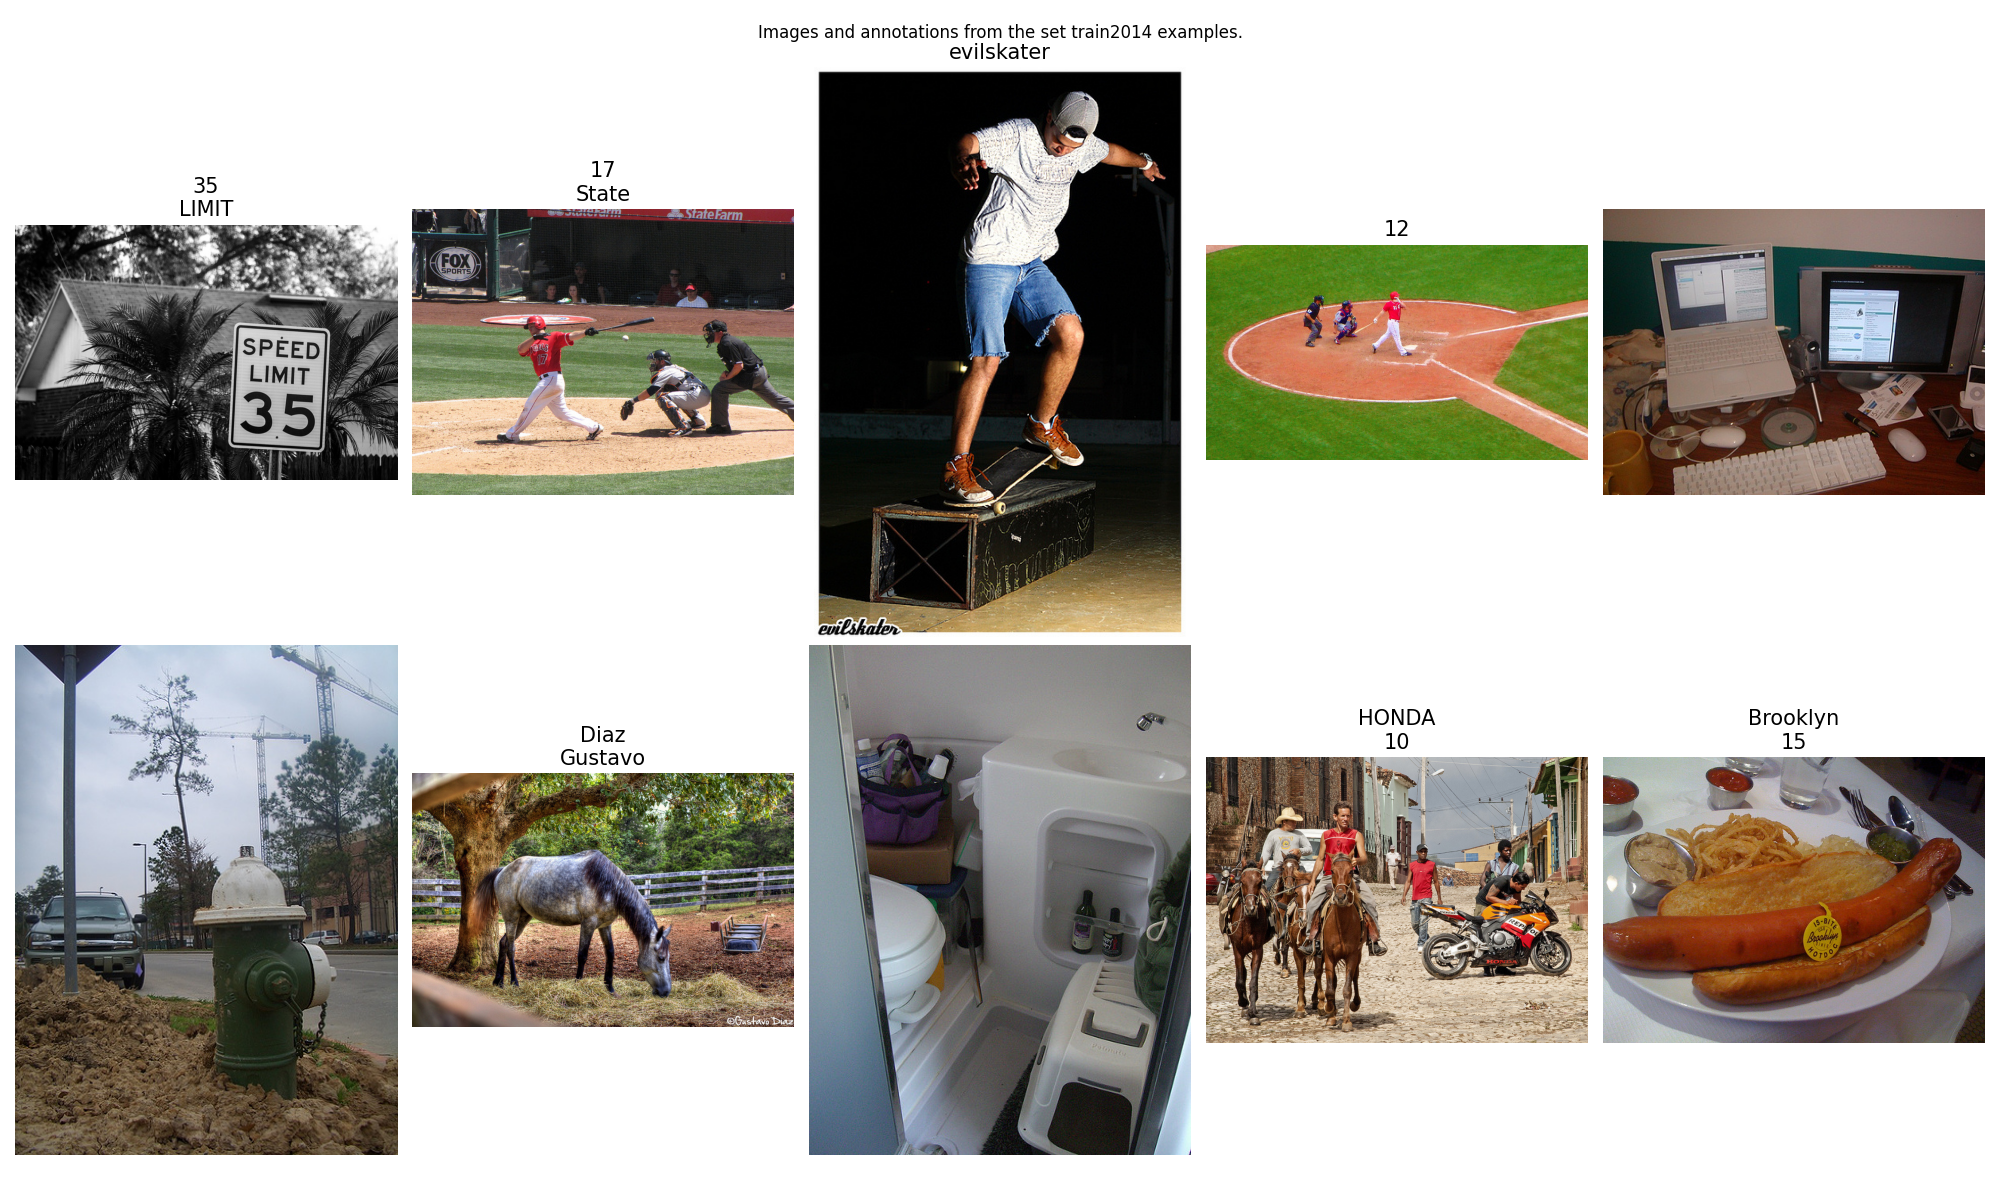
\includegraphics[width=0.8\textwidth]{../reports/figures/visualization_train2014.png} 
    \caption{Subconjunto de entrenamiento.}
    \label{fig:entrenamiento}
\end{figure}

\begin{figure}[ht]
    \centering
    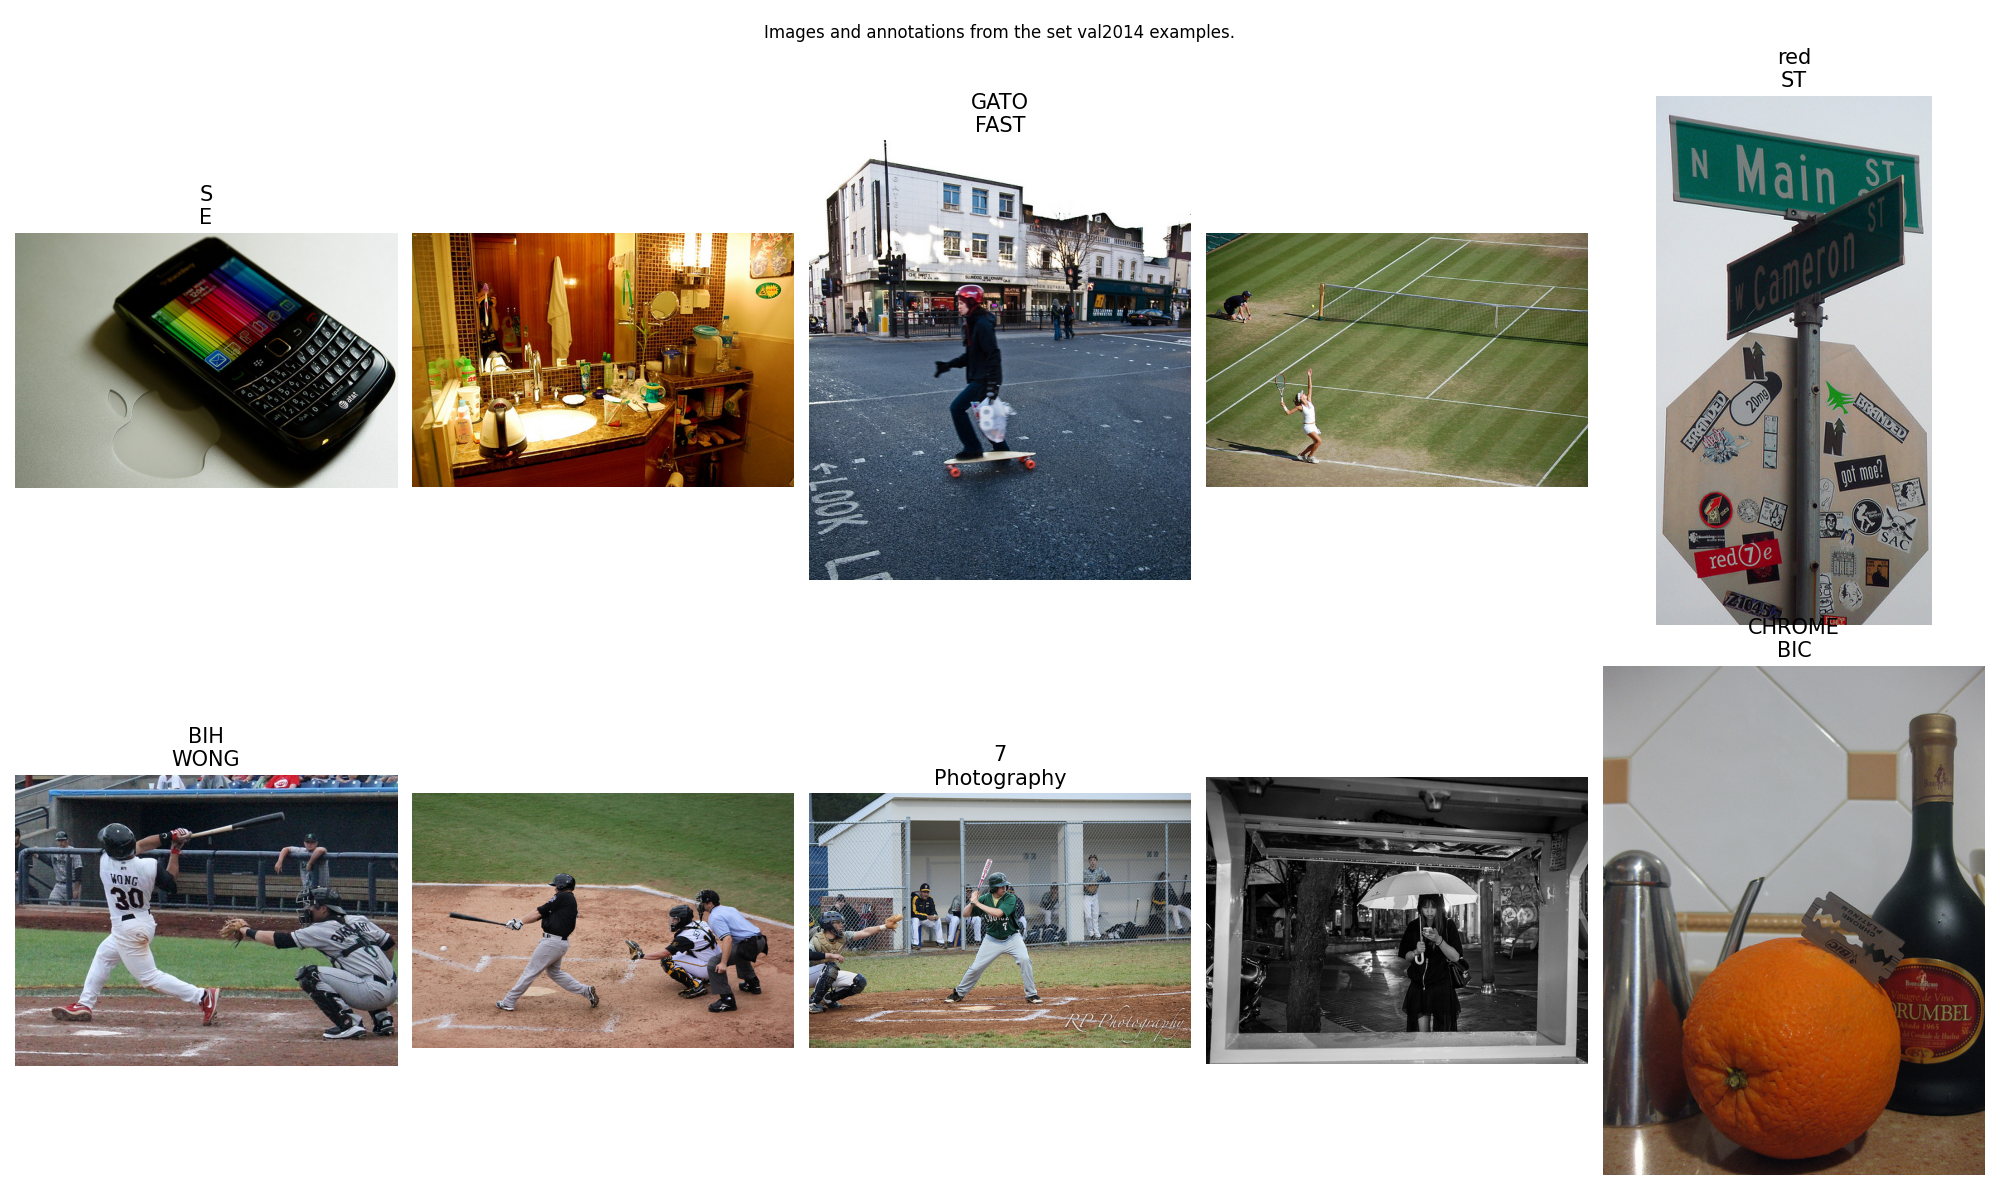
\includegraphics[width=0.7\textwidth]{../reports/figures/visualization_val2014.png} 
    \caption{Subconjunto de validación.}
    \label{fig:validacion}
\end{figure}


\newpage

Se detallan ejemplos de imágenes de las clases \textit{handwritten y machine printed}.

\begin{figure}[ht]
    \centering
    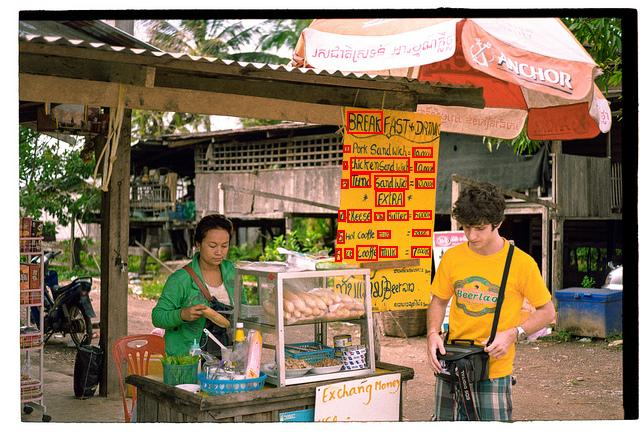
\includegraphics[width=0.7\textwidth]{../reports/figures/example_handwritten.jpg} 
    \caption{Imagen con texto de clase handwritten.}
    \label{fig:handwritten}
\end{figure}

\begin{figure}[ht]
    \centering
    \includegraphics[width=0.5\textwidth]{../reports/figures/example_machine_printed.jpg} 
    \caption{Imagen con texto de clase machine printed.}
    \label{fig:machineprinted}
\end{figure}

\newpage


\subsection{Preprocesamiento}

\begin{itemize}
    \item En el archivo train2014 se dispone de 23.485 imágenes de las cuales se tomaron: 
     \begin{itemize}
        \item Imágenes en subset train: 15656, representa aproximadamente 70\%.
        \item Imágenes en subset val: 7829, representa aproximadamente 30\%.
     \end{itemize}
    \item Se filtraron solo las anotaciones legibles con utf8 string no vacío. 
    \item Recorte y guardado de regiones de texto: Se recorren imágenes anotadas,
     se validan las bounding boxes y se recortan las regiones que contienen texto. 
     Cada recorte se guarda como una imagen PNG en una carpeta de salida.
    \item Generación de archivo de etiquetas: Por cada recorte válido, se registra su nombre de 
    archivo y el texto correspondiente en un archivo labels.csv, listo para ser usado en 
    entrenamiento de modelos OCR.
\end{itemize}

\section{Modelos Encoder-Decoder}

\subsection{Elección de modelos}

Se seleccionaron dos modelos preentrenados basados en ViT que forman parte de la librería 
\textit{transformers} de \textbf{Hugging Face}: \\

El modelo \textbf{TrOCR} \cite{trocr} es un modelo codificador-decodificador, que consiste en un Transformador de imagen 
como codificador y un Transformador de texto como decodificador. El codificador de imagen se 
inicializó a partir de los pesos de BEiT, mientras que el decodificador de texto se inicializó a 
partir de los pesos de RoBERta. 

\begin{itemize}
    \item Identificador: \textit{microsoft/trocr-base-handwritten}.
    \item Arquitectura: ViT + GPT2.
    \item Diseñado para transcripción de texto manuscrito.
    \item Entrenado sobre IAM y similares.
    \item Requiere recortes individuales de texto como entrada.
\end{itemize}
    
\textbf{Donut} \cite{donut} consiste en un codificador de visión (Swin Transformer) y un decodificador de texto (BART).

\begin{itemize}
    \item Identificador: \textit{naver-clova-ix/donut-base}.
    \item Arquitectura: ViT + Decoder.
    \item Diseñado para tareas documentales estructuradas.
    \item OCR-free: no requiere segmentación previa.
    \item Entrada: imagen completa. Salida: JSON estructurado con todos los textos.
\end{itemize}

\subsection{Fine-tuning}

Los modelos preentrenados fueron entrenados en dominios diferentes (documentos, manuscritos, formularios), 
COCO-Text representa escenas en contextos naturales (carteles, letreros, callejeros). El objetivo de aplicar
fine-tuning es que permite adaptar el conocimiento del modelo a este nuevo dominio visual y textual. Este proceso
es fundamental para mejorar la capacidad del modelo de generalizar sobre este nuevo tipo de datos.


\subsection{Cuestiones de diseño}

\begin{itemize}
    \item TrOCR: Se usaron recortes individuales (regiones de texto) para aprovechar el diseño del modelo orientado a transcripción.
    Cada imagen se asocia a un string objetivo (utf8-string).
    \item Donut: Se usaron imágenes completas. Para cada imagen, se generó un target-json que concatena o estructura los textos anotados como respuesta.
    Se aprovechó su arquitectura OCR-free para evaluar su desempeño en tareas de document understanding.
\end{itemize}


\section{Visualizaciones}

Para analizar el comportamiento del modelo TrOCR, se extrajeron los mapas de atención de cada token generado:

\begin{itemize}
    \item Se generó el mapa de atención del primer token.
    \item Se generaron secuencias paso a paso mostrando atención por token.
    \item Se superpusieron los mapas sobre la imagen original recortada.
\end{itemize}

Esto permitió observar cómo el modelo enfoca su atención en distintas partes del texto a medida que genera cada caracter.

A continuación se detallan imagenes que ilustran como el modelo realiza el proceso de atención para distintos textos.

\begin{figure}[H]
    \centering
    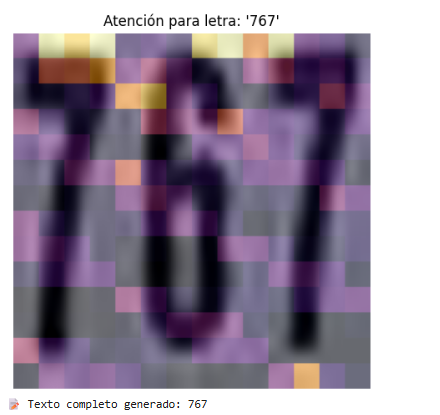
\includegraphics[width=0.8\textwidth]{../reports/figures/attention_heatmap3.png} 
    \caption{Ejemplo 1 TrOCR attention.}
    \label{fig:attention1}
\end{figure}

\clearpage  % Fuerza el vaciado de la cola de figuras y salto de página


\begin{figure}[H]
    \centering
    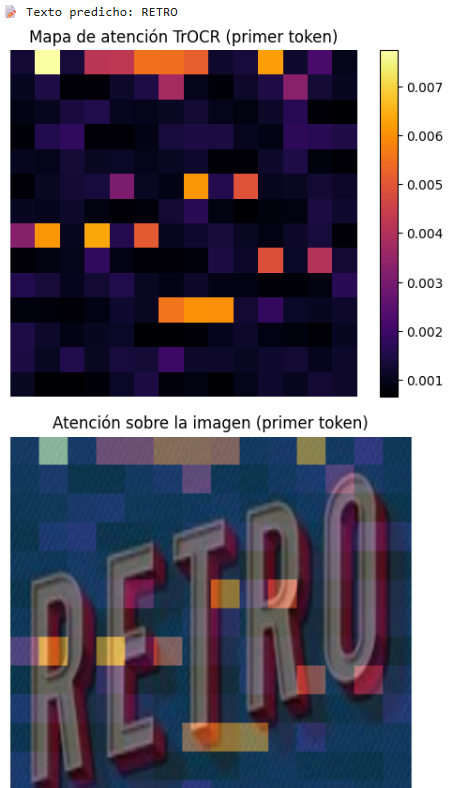
\includegraphics[width=0.7\textwidth]{../reports/figures/attention_heatmap2.png} 
    \caption{Ejemplo 2 TrOCR attention.}
    \label{fig:attention2}
\end{figure}


\section{Resultados}

\subsection{Métricas}

El Character Error Rate (CER) es una métrica utilizada para evaluar el rendimiento 
de modelos de reconocimiento óptico de caracteres (OCR). Representa la proporción
de caracteres que fueron incorrectamente reconocidos, calculada como la suma de 
inserciones, eliminaciones y sustituciones necesarias para transformar la 
predicción en la transcripción correcta, dividida por la cantidad total de 
caracteres de referencia. Un valor de CER más bajo indica un mejor desempeño 
del modelo.


A continuación, se detalla la tabla de la comparación los modelos Donut y TrOCR sobre el conjunto de datos de test:
\begin{table}[h!]
\centering
\begin{tabular}{|l|l|l|l|c|c|c|}
\hline
\textbf{Modelo}  & \textbf{Entrada} & \textbf{Salida} & 
\textbf{Accuracy} & \textbf{CER} & \textbf{Exact Match} \\
\hline
TrOCR & Imagen recortada & Texto plano & 0.6717 & 0.3283 & 0.4726 \\
Donut & Imagen completa & JSON estructurado & 0.1795 & 0.8909 & 0.0706 \\
\hline
\end{tabular}
\caption{Comparación entre los modelos TrOCR y Donut.}
\label{tab:model-comparison}
\end{table}


\subsection{Análisis de los resultados}

\begin{table}[h!]
\centering
\begin{tabular}{|p{6cm}|p{6cm}|}
\hline
\textbf{TrOCR} & \textbf{Donut} \\
\hline
\begin{itemize}
    \item CER promedio: ~32.8\%
    \item Predicciones precisas en recortes bien centrados y legibles
    \item Sensible a ruido o palabras rotadas
\end{itemize}
&
\begin{itemize}
    \item Predicciones razonables en contexto global
    \item Más robusto frente a textos múltiples o estructurados
    \item Requiere cuidado en el formato del JSON objetivo
\end{itemize}
\\
\hline
\end{tabular}
\caption{Comparación entre TrOCR y Donut.}
\label{tab:ventajas}
\end{table}


\section{Conclusiones}

Se pudo demostrar que ambos modelos resultan aplicables de manera efectiva a tareas de 
reconocimiento óptico de caracteres (OCR) sobre el conjunto de datos COCO-Text. En particular,
TrOCR se mostró más adecuado para tareas de transcripción directa en regiones de texto 
aisladas, mientras que Donut evidenció ventajas en escenarios donde es necesario interpretar 
la imagen en su totalidad o generar salidas estructuradas.
Asimismo, el proceso de fine-tuning resultó fundamental para alcanzar desempeños 
satisfactorios, dada la divergencia existente entre el dominio de los datos originales y
las características específicas del dataset utilizado.

\section{Futuras mejoras}

Consideramos que se podrían aplicar distintas tareas para la futura mejora de los modelos, a continuación
se detallan algunas de ellas:

\begin{itemize}
    \item Aumentar el tamaño del dataset de entrenamiento.
    \item Aplicar data augmentation sobre los recortes.
    \item Usar métricas más precisas como WER (Word Error Rate) \cite{wer}.
    \item Explorar adaptaciones de Donut a OCR en escena natural (prompting o instrucción).
\end{itemize}

\begin{thebibliography}{9}

\bibitem{trocr}
Li, M., Yin, F., Zhang, C., \& Liu, C. (2021). TrOCR: Transformer-based Optical Character Recognition with Pre-trained Models. \textit{arXiv preprint arXiv:2109.10282}.  
Disponible en: \url{https://huggingface.co/microsoft/trocr-base-handwritten}

\bibitem{donut}
Kim, G., Kim, Y., Cho, S., \& Park, S. (2022). Donut: Document Understanding Transformer without OCR. \textit{arXiv preprint arXiv:2111.15664}.  
Disponible en: \url{https://huggingface.co/naver-clova-ix/donut-base}

\bibitem{cocotext}
Veit, A., Matera, J., Neumann, L., Matas, J., \& Belongie, S. (2016). COCO-Text: Dataset and Benchmark for Text Detection and Recognition in Natural Images.  
Disponible en: \url{https://bgshih.github.io/cocotext/}

\bibitem{coco2014}
Lin, T.-Y., Maire, M., Belongie, S., et al. (2014). Microsoft COCO: Common Objects in Context.  
Disponible en: \url{https://cocodataset.org/#download}

\bibitem{wer}
Wikipedia contributors. (s.f.). Word error rate. Wikipedia.  
Disponible en: \url{https://en.wikipedia.org/wiki/Word_error_rate}

\end{thebibliography}


\end{document}
